\documentclass[a4 paper]{article}
\usepackage{tikz-qtree}
% Set target color model to RGB
\usepackage[inner=1.75cm,outer=1.75cm,top=2.5cm,bottom=2.5cm]{geometry}
\usepackage{setspace}
\usepackage[rgb]{xcolor}
\usepackage{verbatim}
\usepackage{subcaption}
\usepackage{amsgen,amsmath,amstext,amsbsy,amsopn,tikz,amssymb,tkz-linknodes}
\usepackage{fancyhdr}
\usepackage[colorlinks=true, urlcolor=blue,  linkcolor=blue, citecolor=blue]{hyperref}
\usepackage[colorinlistoftodos]{todonotes}
\usepackage{rotating}
%\usetikzlibrary{through,backgrounds}
\hypersetup{%
pdfauthor={Ashudeep Singh},%
pdftitle={Homework},%
pdfkeywords={Tikz,latex,bootstrap,uncertaintes},%
pdfcreator={PDFLaTeX},%
pdfproducer={PDFLaTeX},%
}
%\usetikzlibrary{shadows}
% \usepackage[francais]{babel}
\usepackage{booktabs}
\usepackage{fancyhdr}

\newcommand{\ra}[1]{\renewcommand{\arraystretch}{#1}}

\newtheorem{thm}{Theorem}[section]
\newtheorem{prop}[thm]{Proposition}
\newtheorem{lem}[thm]{Lemma}
\newtheorem{cor}[thm]{Corollary}
\newtheorem{defn}[thm]{Definition}
\newtheorem{rem}[thm]{Remark}
\numberwithin{equation}{section}

\newcommand{\homework}[8]{
   \pagestyle{fancy}
   \thispagestyle{plain}
   \newpage
   \setcounter{page}{1}
   \noindent
   \begin{center}
   \framebox{
      \vbox{\vspace{2mm}
    \hbox to 6.78in { { CS345:~Algorithms - II \hfill {\small #2}} }
       \vspace{6mm}
       \hbox to 6.78in { {\Large \hfill \bf#1  \hfill} }
       \vspace{6mm}
       \hbox to 6.78in { {\large {Name: {\rm \textbf{#3}}}}{\hfill {Instructor: #6}}}
       \vspace{2mm}
       \hbox to 6.78in { {\large {Roll-No: {\rm \textbf{#4}}}}{\hfill TA: #5}}
       \vspace{2mm}
       \hbox to 6.78in { {{Email: {\rm #7}}}{\hfill TA's Email: #8}  }
       \vspace{2mm}
       \hbox to 6.78in { {\large{\hfill Max Points: 50}} }
       \vspace{2mm}
      \vspace{2mm}}
   }
   \end{center}
   \fancyhf{}
    \fancyhead[LE,RO]{{CS345:~Algorithms - II}}
    \fancyhead[RE,LO]{{#3 -- #4}}
    \fancyfoot[CE,CO]{Page: \thepage}
    \fancyfoot[LE,RO]{{#1}}
   \renewcommand{\headrulewidth}{1pt}
   \renewcommand{\footrulewidth}{1pt}
   \vspace*{4mm}
}

\newcommand{\problem}[2]{~\\\fbox{\bf\large{#1}}\hfill [#2]\newline\newline}
\newcommand{\subproblem}[1]{~\\\fbox{\textbf{Sub - Problem #1}}\newline\newline}
\newcommand{\D}{\mathcal{D}}
\newcommand{\Hy}{\mathcal{H}}
\newcommand{\VS}{\textrm{VS}}
\newcommand{\solution}{~\newline\textbf{\textit{(Solution)}} }

\newcommand{\bbF}{\mathbb{F}}
\newcommand{\bbX}{\mathbb{X}}
\newcommand{\bI}{\mathbf{I}}
\newcommand{\bX}{\mathbf{X}}
\newcommand{\bY}{\mathbf{Y}}
\newcommand{\bepsilon}{\boldsymbol{\epsilon}}
\newcommand{\balpha}{\boldsymbol{\alpha}}
\newcommand{\bbeta}{\boldsymbol{\beta}}
\newcommand{\0}{\mathbf{0}}
\usepackage[linesnumbered,lined,boxed,commentsnumbered]{algorithm2e}
\include{pythonlisting}
\newcommand{\forcond}{$i=0$ \KwTo $n$}



\begin{document}
\homework{Assignment \#2}{Due: 13/09/19}{Ayush Hitesh Soneria}{170192}{Pranav Bisht}{Prof. Nitin Saxena}{ayushhs@iitk.ac.in OR ayushhs@cse.iitk.ac.in}{pbisht@cse.iitk.ac.in}

\problem{Question 1: MinGap of Set}{6 points}
We will design a tree structure as an augmented AVL tree. Every node in this tree will have the following fields:
Augmentation (w.r.t to each node, say v) as follows:
\begin{itemize}
  \item[\textendash] left: pointer to left child of v
  \item[\textendash] right: pointer to right child of v
  \item[\textendash] key: number stored in the v
  \item[\textendash] maxkey: maximum key in the subtree rooted at v
  \item[\textendash] minkey: minimum key in the subtree rooted at v
  \item[\textendash] mingap: minimum positive difference in the subtree rooted at v
\end{itemize}
The 3 additional fields, maxkey, minkey and mingap need to be updated for insertion and deletion operations without increasing time complexity which is O(logn). Hence we will do the update them recursively: \\\\
\begin{algorithm}[H]
\SetAlgoLined
\KwData{$v \leftarrow $ {node to be inserted or deleted}}
\tcc{In this algorithm we are using minimum function which gives minimum of all its arguments}
INT\_MAX $\leftarrow $ {Maximum possible integer in a computer}\;
\If{node v has no children}
{   
    v.maxkey = v.key\;
    v.minkey = v.key\;
    v.mingap = INT\_MAX\;
}
\ElseIf{node v has no right child}
{
    v.maxkey = v.key\;
    v.minkey = v.left.minkey\;
    v.mingap = minimum(INT\_MAX, v.left.mingap, v.key-v.left.maxkey)\;
}
\ElseIf{node v has no left child}
{
    v.maxkey = v.right.maxkey\;
    v.minkey = v.key\;
    v.mingap = minimum(INT\_MAX, v.right.mingap, v.right.minkey-v.key)\;
}
\Else(\tcc*[f]{both children present})
{
    v.maxkey = v.right.maxkey\;
    v.minkey = v.left.minkey\;
    v.mingap = minimum(v.right.mingap, v.right.minkey-v.key, v.left.mingap, v.key-v.left.maxkey)\;
}
\caption{updation for standard tree operations in $O(logn)$}
\end{algorithm}
\vspace{4mm}
\newpage
\problem{Question 1: Continued}{6 points}
\underline{\textsc{Proof of Correctness \& Analysis}}\\\\
We need maxkey and minkey in addition to mingap is because we need to also include the node.key itself in our calculations when getting mingap, not just its subtree's mingaps. So we now can also include v.right.minkey-v.key and v.key-v.left.maxkey in finding mingap of v.\\ 
During standard insertions and deletions in order to balance AVL tree height rotations may be done. The above algorithm needs to be implemented on the two rotated nodes. As we can see atmost O(1) such rotations may be done, and only the nodes in the path from updated nodes to root have to be updated as well. Meaning we will have to update only O(logn) nodes with above algorithms which itself runs in O(1) time. Hence updation for standard tree operations is done in O(logn) with our augmented AVL tree.\\
Once the elements of set T are inserted in augmented AVL tree (pre-processing) then MinGap(T) is mingap field of the root of AVL tree, hence MinGap(T) can be done in O(1).\\\\
\problem{Question 2: Orthogonal Range Search}{5 points}
As seen in class for Orthogonal Range Search, we use an augmented AVL tree, Xtree, where each node v contains the x-coordinate value and an AVL tree w.r.to y-coordinates, Ytree(v). The Ytree(v) is not augmented, it only contains the y-coordinate in our implementation done in class.\\
But let us modify our algorithm, suppose now we augment the Ytrees as well, with a size field stored in each node of the Ytree. The size field of a node v,  will contain the sum of number of nodes in subtrees of v. Hence now we can tweak the pseudo-code discussed in class to get required output as follows:\\
Suppose given rectangle coordinates are (x1,y1) and (x2,y2). In Xtree suppose node of x1 is s and node of x2 is t. Let p be the LCA(lowest common ancestor) of s and t. We need the points which lie between x1 and x2, as well as y1 and y2.\\\\
\underline{\textsc{Pseudo-code}}\\\\
\begin{algorithm}[H]
\SetAlgoLined
\KwData{$Xtree \leftarrow $ {Augmented AVL tree with x-coordinates and Ytrees}}
\KwData{$Ytree \leftarrow $ {Augmented AVL tree with y-coordinates and size}}
\KwResult{Number of points in a given rectangle}
\SetKwFunction{FRecurs}{Count(T,x1,x2,y1,y2)}%
\SetKwProg{Fn}{Function}{:}{}
\Fn{\FRecurs}
{
int ans=0\;
\If{right child of s is not NULL}{
\tcc{checking for blue nodes and blue subtrees as discussed in class}
ans += the number of nodes in s.right.Ytree between y1 and y2 using size field\;
\tcc{to know which nodes are between y1 and y2, do RangeSearch(Ytree,y1,y2) as discussed in class and keep a counter using the size field,will take O(logn)}}
\While(\tcc*[f]{traverse from s to LCA}){s is not equal to p}{
\If{s is left child of its parent}{\tcc{checking for blue nodes and blue subtrees as discussed in class}
ans += the number of nodes in s.parent.Ytree and s.parent.right.Ytree between y1 and y2 using size field\;
\tcc{to know which nodes are between y1 and y2, do RangeSearch(Ytree,y1,y2) as discussed in class and keep a counter using the size field,will take O(logn)}
}
s = s.parent\;
}
similarly for path t to p\;
return ans\;
}
\textbf{End Function}
\caption{Orthogonal Range Count in $O(log^{2}n)$}
\end{algorithm}
\vspace{4mm}
\newpage
\problem{Question 2: Continued}{5 points}
\underline{\textsc{Proof of Correctness \& Analysis}}\\\\
After insertion/deletions of a node in AVL, the tree can become height unbalanced. In order to balance it, rotations may be necessary. During rotations, all the fields of the node have to be carefully updated, especially the size field. Right-Rotate(y):
$$x = y.left$$
$$y.size = y.left.size + y.right.size $$
$$x.size = x.left.size + x.right.size $$
So rotations take O(1) time, also standard tree operations can be done on the Ytree in O(logn) time as only size field updation required. The two while loops in the algorithm itself have O(logn) iterations and in each iteration RangeSearch(Ytree,y1,y2) will take O(logn), hence time complexity of Orthogonal Range Count is $O(log^{2}n)$.\\\\
\problem{Question 3: Data Structure that stores Sequence of Numbers}{13 points}
The data structure D we will design will be an augmented AVL tree, which will perform store sequence of numbers and do the asked operations in O(logn) time. \\
We will store the following fields in each node in D:\\
Augmentation (w.r.t to each node, say v) as follows:
\begin{itemize}
  \item[\textendash] left: pointer to left child of v
  \item[\textendash] right: pointer to right child of v
  \item[\textendash] parent: pointer to parent of v
  \item[\textendash] value: number stored in the v
  \item[\textendash] size: size of subtree rooted at v
  \item[\textendash] minsub: minimum value in the subtree rooted at v
\end{itemize}
Let us initialize the the fields in tree D (pre-processing). The left,right,parent and value fields are trivial and should be stored such that when the general InOrder Traversal is applied to D, the output is the sequence of numbers remembering the array order. We will initialise the min and size fields recursively:\\\\
if node v is leaf then v.minsub = v.value, else 
$$v.minsub = min(v.value, v.left.minsub, v.right.minsub)$$
if node v is leaf then v.size = 1, else
$$v.size = v.left.size + v.right.size + 1$$
\subproblem{(1): Insert(D,i,x)}
Please look at Algorithm for Insert(D,i,x) on next page before going through analysis given next.\\\\
\underline{\textsc{Proof of Correctness \&  Analysis}}\\\\
After insertion of a node in AVL, the tree can become height unbalanced. In order to balance it, rotations may be necessary. During rotations, all the fields of the node have to be carefully updated, especially the size and minsub fields (given on next page).\\
This algorithm is very similar to the insertion algorithm in a normal AVL tree whose complexity if O(logn). During balancing, extra field updating also will take only O(logn) time as O(1) update operations have to be performed for O(logn) nodes. Hence the time complexity of Insert(D,i,x) algorithm is O(logn).\\
\newpage
\problem{Question 3: Continued}{13 points}
Update during Right-Rotate(y):\\
$$x = y.left$$
$$y.size = y.left.size + y.right.size + 1$$
$$x.size = x.left.size + x.right.size + 1$$
$$y.minsub = min(y.value, y.left.minsub, y.right.minsub)$$
$$x.minsub = min(x.value, x.left.minsub, x.right.minsub)$$
\\Similarly for left-rotate, also here we take size(NULL)=0 and minsub(NULL)=0. We can see here that balancing during single rotation will take O(1) time. \\\\
\subproblem{(1): Insert(D,i,x): Pseudo-code}
\begin{algorithm}[H]
\SetAlgoLined
\KwData{$D \leftarrow $ {Augmented initialized AVL tree}}
\KwData{$root \leftarrow $ {root of D}}
\KwResult{updated D after insertion of x at i-th location}
\SetKwFunction{FRecurs}{Insert(root,i,x)}%
\SetKwProg{Fn}{Function}{:}{}
\Fn(\tcc*[f]{algorithm as a recursive function}){\FRecurs}
{
    \If{(root == NULL)}
    {   
        $p \leftarrow $ {allocate new node}\;
        p.left = NULL\;
        p.right = NULL\;
        p.parent = NULL\;
        p.value = x\;
        p.size = 1\;
        p.minsub = x\;
        return p\;
    }
    \Else
    {   
        root.size = root.size + 1\;
        \If{(root.minsub $>$ x)}
        {
            root.minsub = x\;
        }
        \uIf{(root.left == NULL)}
        {
             $a \leftarrow $ 0\;
        }
        \Else(\tcc*[f]{})
        {
            $a \leftarrow $ root.left.size\;
        }
        \uIf{(i $<=$ a+1)}
        {
             root.left = Insert(root.left,i,x)\;
             root.left.parent = root\;
        }
        \Else(\tcc*[f]{})
        {
            root.right = Insert(root.right,i-a-1,x)\;
            root.right.parent = root\;
        }
        return root\;
    }
}
\textbf{End Function}\\
\textbf{Balance the Tree if it turns out to be unbalanced}
\caption{Insert(D,i,x) in $O(logn)$}
\end{algorithm}
\vspace{4mm}
\newpage
\subproblem{(2): Delete(D,i): Pseudo-code}
\begin{algorithm}[H]
\SetAlgoLined
\KwData{$D \leftarrow $ {Augmented initialized AVL tree}}
\KwData{$root \leftarrow $ {root of D}}
\KwResult{updated D after Deletion of x at i-th location}
\SetKwFunction{FRecurs}{Delete(root,i)}%
\SetKwProg{Fn}{Function}{:}{}
\Fn(\tcc*[f]{algorithm as a iterative function}){\FRecurs}
{
    \If{(root == NULL)}
    {   
        return\;
    }
    $p \leftarrow $ {node storing i-th element}\;
    \uIf{(p.left $!=$ NULL) and (p.right $==$ NULL)}
    {
        \uIf{(p.parent.right $==$ p)}
        {
            p.parent.right = p.left\;
        }
        \Else
        {
            p.parent.left = p.left\;
        }
    }
    \uElseIf{(p.left $==$ NULL) and (p.right $!=$ NULL)}
    {
         \uIf{(p.parent.right $==$ p)}
        {
            p.parent.right = p.right\;
        }
        \Else
        {
            p.parent.left = p.right\;
        }
    }
    \uElseIf{(p.left $==$ NULL) and (p.right $==$ NULL)}
    {
        \uIf{(p.parent.right $==$ p)}
        {
            p.parent.right = NULL\;
        }
        \Else
        {
            p.parent.left = NULL\;
        }
    }
    \Else(\tcc*[f]{need to find successor of p})
    {
        q = p.right\;
        \While{(q.left $!=$ NULL)}
        {
            q.size = q.size - 1\tcc*[r]{need to update size field in path from p to successor of p}
            q = q.left\;
        }
        p.value = q.value\;
        q.parent.left = q.right\tcc*[r]{delete node q}
        \If{(q.right $!=$ NULL)}
        {
            q.right.parent = q.parent.left\;
        }
        q = q.parent\;
        \While(\tcc*[f]{need to update minsub field in path from p to successor of p}){(q $!=$ p)}
        {
            q.minsub = minimum(q.value,q.left.minsub,q.right.minsub)\;
            q = q.parent\;
        }
    }
    \While(\tcc*[f]{need to update minsub and size fields in path from p to root}){(p $!=$ root)}
        {
            p.size = p.size - 1\;
            p.minsub = minimum(p.value,p.left.minsub,p.right.minsub)\;
            p = p.parent\;
        }
        root.size = root.size - 1\tcc*[r]{update root as well}
        root.minsub = minimum(root.value,root.left.minsub,root.right.minsub)\;
        return root\;
}
\textbf{End Function}\\
\caption{Delete(D,i) in $O(logn)$}
\end{algorithm}
\vspace{1mm}
\newpage
\problem{Question 3: Continued}{13 points}
\subproblem{(3): Delete(D,i): Continued}
\underline{\textsc{Proof of Correctness \& Analysis}}\\\\
When the node p to be deleted has one or zero children, then trivial case. Just update the fields of minsub and size in the path from deleted node to root. When node p has two children then find successor (decrement size values along path of p to successor) and replace the value of p. Then delete successor node and replace minsub values from successor to p. Then update the fields of minsub and size in the path from p to root.\\\\ Finding successor will be O(logn) time. The two updation while loops will have max of log n iterations as there can be iterations = height of tree at max. Also just like insertion, balancing tree might be needed after deletion which again would take O(logn) time.\\ Hence time complexity of Delete(D,i) is O(logn).\\\\
\subproblem{(3): Report(D,i)}
\underline{\textsc{Pseudo-code}}\\\\
\begin{algorithm}[H]
\SetAlgoLined
\KwData{$D \leftarrow $ {Augmented initialized AVL tree}}
\KwResult{Number at i-th locations}
\SetKwFunction{FRecurs}{Report(D,i)}%
\SetKwProg{Fn}{Function}{:}{}
\Fn(\tcc*[f]{algorithm as a iterative function}){\FRecurs}
{
$root \leftarrow $ {root of D}\;
$check \leftarrow $ 0\; 
\While{(check == 0)}{
\uIf{(root.left == NULL)}
{
     $a \leftarrow $ 0\;
}
\Else(\tcc*[f]{})
{
$a \leftarrow $ root.left.size\;
}
\uIf{(i $==$ a+1)}
{
    $check \leftarrow $ 1\; 
}
\uElseIf(\tcc*[f]{}){(i $>$ a+1)}
{
i = i - a - 1\;
root = root.right\;
}
\Else{
root = root.left\;
}
}
return root.value;
}
\textbf{End Function}
\caption{Report(D,i) in $O(logn)$}
\end{algorithm}
\vspace{4mm}
\underline{\textsc{Proof of Correctness \& Analysis}}\\\\
We are traversing some path from root down to the i-th location. The maximum we can traverse by taking any path in a tree is the height of the tree which is equal to log n.\\ Hence time complexity of Report(D,i) is O(log n).\\
\newpage
\problem{Question 3: Continued}{13 points}
\subproblem{(4): Min(D,i,j)}
\underline{\textsc{Pseudo-code}}\\\\
\begin{algorithm}[H]
\SetAlgoLined
\KwData{$D \leftarrow $ {Augmented initialized AVL tree}}
\KwResult{Smallest number from the i-th to the j-th locations}
\SetKwFunction{FRecurs}{Min(D,i,j)}%
\SetKwProg{Fn}{Function}{:}{}
\Fn(\tcc*[f]{algorithm as a iterative function}){\FRecurs}
{
\tcc{In this algorithm we are using minimum function which gives minimum of all its arguments}
$s \leftarrow $ {node storing ith element}\;
$t \leftarrow $ {node storing jth element}\;
$lca \leftarrow $ {lowest common ancestor (LCA) of s and t}\tcc*[r]{this step takes O(logn) time}
\If{(s != lca)}
{
m1 = s.value\tcc*[r]{m1 will store the minimum value on left side of lca}
\If{(s.right $!=$ NULL)}
{
    m1 = minimum(m1, s.right.minsub)\;
}
\While(\tcc*[f]{we traverse from s to lca}){(s.parent $!=$ lca)}{
    \If{(s == s.parent.left)}
    {
        \tcc{positions of s.parent and subtree s.parent.right belong in range i to j}
        m1 = minimum(m1, s.parent.value, s.parent.right.minsub)\;   
    }
    s = s.parent\;
}
}
\If{(t != lca)}
{
m2 = t.value\tcc*[r]{m2 will store the minimum value on right side of lca}
\If{(t.left $!=$ NULL)}
{
    m2 = minimum(m2, t.left.minsub)\;
}
\While(\tcc*[f]{we traverse from t to lca}){(t.parent $!=$ lca)}{
    \If{(t == t.parent.right)}
    {
        \tcc{positions of t.parent and subtree t.parent.left belong in range i to j}
        m2 = minimum(m2, t.parent.value, t.parent.left.minsub)\;   
    }
    t = t.parent\;
}
}
return minimum(m1, m2, lca.value)\tcc*[r]{Required Output}
}
\textbf{End Function}
\caption{Min(D,i,j) in $O(logn)$}
\end{algorithm}
\vspace{4mm}
\underline{\textsc{Proof of Correctness \& Analysis}}\\\\
In the algorithm we only consider nodes (and their right subtrees) whose left child is in the path from LCA to s and the nodes (and their left subtrees) whose right child is in the path from LCA to t. One can easily visualize these nodes and subtrees lie between s and t. Meaning these nodes and subtrees will contain values which lie between the i-th (node s) and j-th (node t) locations. Hence the minimum value which we obtain is provably correct.\\\\
The two while loops in the algorithm take O(logn) time because maximum traversal can be from leaf to root, which has height log n. Finding out the LCA also takes O(logn) time. Hence time complexity of Min(D,i,j) is O(logn).
\newpage
\problem{Question 4: Overlapping Rectangles}{12 points}
\underline{\textsc{Algorithm}}\\\\
\begin{algorithm}[H]
\SetAlgoLined
\KwData{$n \leftarrow $ {number of rectangles}}
\KwData{$x1,x2,y1,y2 \leftarrow $ {coordinates of each given rectangles}}
Store the y-coordinates (y1,y2) of all rectangles in an array, A. So A will have 2n elements\\
Associate fields (maybe using pointers or structs), color and id with each element, s.t. if y-coordinate is lower edge of its rectangle then color will be blue else color red and id will be unique number distinguishing each rectangle coordinates from others (each rectangle will be given a unique id when taken as input)\\
Sort (in non-decreasing order) the array A according to its y-coordinate value\\
Create a empty augmented balanced BST such as augmented AVL tree, say T\\
T will take as input x-coordinates of rectangles as keys and will also keep a count field which will be zero initially\\
Start \textbf{vertical line sweep} from bottom, meaning start iteration from first element of A (horizontal rectangle edge with least y-coordinate)\\
Here we implement a \textbf{while loop} such that if we ever see the red edge of last element of A (horizontal rectangle edge with highest y-coordinate), we break loop\\
Every time we come across a \textbf{blue edge} of rectangle R (identified using id of edge from A), insert x1 and x2 of R into T\\
Also increment (++) count field in the nodes of T which are between the x1,x2 of R \\
We also need to keep a variable, \textbf{MX}, which keeps the maximum out of all the node's (maximum attained) count fields\\
Every time we come across a \textbf{red edge} of rectangle R (identified using id of edge from A), delete x1 and x2 of R from T\\
Also decrement (- -) count field in the nodes of T which are between the x1,x2 of R \\
To check the nodes which are between x-coordinates of R we first find the LCA (lowest common ancestor) of x1,x2 and then looking at suitable ancestors and ancestral subtrees (as done in class or even in Q3. sub-problem 4) we update count field as needed\\
Our output will be MX once the loop breaks\\
\caption{Maximum overlapping rectangles at any point in $O(nlogn)$}
\end{algorithm}
\vspace{4mm}
Here algorithm written in words, because pseudo-code would be unnecessarily complex to explain\\\\
\underline{\textsc{Proof of Correctness \& Analysis}}\\\\
The fields augmented in T, do not make the insert and delete time complexity of T different from standard AVL tree insert/delete time which is O(logn) time. This is because the count field doesn't depend on any other nodes in the tree. It only increments or decrements based on its location w.r.to the nodes being inserted or deleted and hence insertion/deletion do not have to take special care of count field. (unlike size field like we saw in Q3)\\
\\
The while loop implemented in the algorithm above does 2n iterations as A contains 2n elements.\\
Lines 9 and 12 using method from line 13 (as we have seen in Q3), will take O(logn) time.\\ 
Line 10 happens hand-in-hand with lines 9 and 12.\\
Lines 8 and 11 are insert and delete operations which also take O(logn) time.\\
So for each iteration of while loop takes O(logn) time. Hence the while loop overall takes O(nlogn) time.\\
Sort in line 3 takes O(nlogn) time also.\\
Hence the time complexity of maximum number of rectangles that overlap at any point (maximized over all points in the plane) is O(nlogn) time.\\
\newpage
\problem{Question 5: Synchronized Circuit}{14 points}
\subproblem{1}
Terminology used here,\\
FL(P,N) : final delay (after synchronization) incurred from node P to a leaf node N.\\
MaxDL(P) : Maximum delay which can be incurred from node P to any leaf node.\\
P.left.DL : Delay incurred by the left subtree of P.\\
P.right.DL : Delay incurred by the right subtree of P.\\\\
To establish a greedy approach, let us look at a smaller instance of the problem. Let us look at the smaller tree of two sibling leaf nodes, say N \& M, and their common parent, say P.
\tikzset{every tree node/.style={minimum width=2em,draw,rectangle},
         blank/.style={draw=none},
         edge from parent/.style=
         {draw,edge from parent path={(\tikzparentnode) -- (\tikzchildnode)}},
         level distance=1cm}
\begin{center}
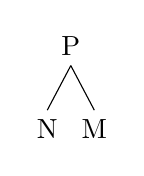
\begin{tikzpicture}
\Tree
[.P     
    [.N ]
    [.M ]
]
\end{tikzpicture}
\end{center}
Suppose before synchronization the delay from P to N is pn, and from P to M is pm. If this tree was synchronized, then FL(P,N) would be equal to FL(P,M). Meaning after some delay enhancement on the edges P to N and P to M, $$FL(P,N) = pn + k_{1} = pm + k_{2} = FL(P,M)$$ Where $k_{1}$ and $k_{2}$ are positive delay enhancements \\
But is it necessary that both $k_{1}$ and $k_{2}$ are needed? Also is this delay enhancement minimum? Let us look into maximum delay from P before synchronization. Suppose, $pn > pm$, then MaxDL(P) = pn. Now when doing delay enhancement, do we necessarily need to enhance pn? What if we only enhanced pm to become pn, that way synchronization is achieved as well as lower delay enhancement done. Meaning we take $k_{1} = 0$ and $k_{2} = pn - pm$. Hence, $$FL(P,N) = pn = pm + (pn - pm) = FL(P,M) = MaxDL(P)$$  So we are reaching a claim here that in the optimal solution, the Max delay from node P before synchronization is equal to Final delay from node P to any leaf node after synchronization. Let us generalize this notion and then prove the claim and that doing delay enhancement this way will indeed give us the optimal solution. \\
\subproblem{2}
Let P be any non-leaf node, which is not synchronized yet, with synchronized left and right subtrees.
\tikzset{every tree node/.style={minimum width=2em,minimum height=2em,draw,rectangle},
         blank/.style={draw=none},
         edge from parent/.style=
         {draw,edge from parent path={(\tikzparentnode) -- (\tikzchildnode)}},
         level distance=1.5cm}
\begin{center}
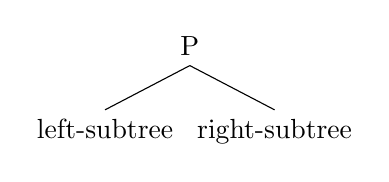
\begin{tikzpicture}
\Tree
[.P     
    [.left-subtree  ]
    [.right-subtree ]
]
\end{tikzpicture}
\end{center}
\textbf{\underline{Claim}}: In the optimal solution, MaxDL(P) = FL(P,N) where N is any leaf node\\
\textbf{\underline{Proof}}: We will try and use contradiction.\\
Let pl be delay on edge P to P.left and pr be delay on edge P to P.right. We can say here that $$MaxDL(P) = Max(P.left.DL + pl, P.right.DL + pr)$$ 
W.l.o.g lets say (P.left.DL + pl) $>$ (P.right.DL + pr) then MaxDL(P) = P.left.DL + pl. Now in the optimal solution, \\if MaxDL(P) $!=$ FL(P,N) [Assumption taken, which is contradictory to our claim]\\ then MaxDL(P) $<$ FL(P,N). Meaning (P.left.DL + pl) $<$ FL(P,N).\\
Let A be any leaf node in left subtree and B be any leaf node in right subtree. Now lets do some delay enhancement in order to make this tree synchronised. $$FL(P,A) = P.left.DL + pl + k_{1} = P.right.DL + pr + k_{2} = FL(P,B).$$ Where $k_{1}$ and $k_{2}$ are positive delay enhancements and we also deduce $k_{2} > k_{1}$\\
\newpage
\problem{Question 5: continued}{14 points}
\subproblem{2: continued}
Looking at both edges of tree, total delay enhancement will be $k_{1}$ + $k_{2}$. But this total delay enhancement isn't minimum, as enhancement of one out of the two edges can clearly be made zero, further reducing enhancement. In doing do so, we are indirectly saying that in order to get minimum enhancement and hence to get optimal solution we need $$k_{1}= 0,k_{2} = (P.left.DL+pl)-(P.right.DL+pr)$$ We can't minimize this enhancement more, as in that case $k_{1}$ would be negative. So taking this enhancement for our optimal solution, gives us that $$FL(P,A) = P.left.DL + pl = P.right.DL + pr + k_{2} = FL(P,B)$$ $$MaxDL(P) = P.left.DL + pl = FL(P,A)$$ Hence we get, $FL(P,N) = MaxDL(P)$ where N is any leaf node.\\ Hence here we reach a contradiction in our assumption that in optimal solution MaxDL(P) $!=$ FL(P,N).\\
Hence our claim is proved. Hence overall we obtain that in the optimal solution, for every non-leaf node P, the minimum delay enhancement = $k_{1} + k_{2} = k_{2} = |(P.lef t.DL+P.left.edge.delay)-(P.right.DL+P.right.edge.delay)|$ This is an important relation we derive here.\\
\subproblem{3}
\underline{\textsc{Pseudo-code}} (we will use the relation derived above)\\\\
\begin{algorithm}[H]
\SetAlgoLined
\KwData{P $\leftarrow$ root of T (given complete binary tree), Global variable: D=0}
\KwResult{Synchronized T and Minimum Total Delay Enhancement in D}
\SetKwFunction{FRecurs}{Enhance}%
\SetKwProg{Fn}{Function}{:}{}
\Fn(\tcc*[f]{algorithm as a recursive function}){\FRecurs{P}}
{
\uIf(\tcc*[f]{reached end of path}){P is a leaf node}{
return 0\;
}
\Else{
$edgeDelay_{P.left} \leftarrow $ {delay on edge between P and P.left}\;
$edgeDelay_{P.right} \leftarrow $ {delay on edge between P and P.right}\;
\tcc{following 2 Variables store minimum enhanced Delay incurred on left and right side of P and P's edge delays}\\
$P.left.DELAY = edgeDelay_{P.left} + Enhance(P.left)$\;
$P.right.DELAY = edgeDelay_{P.right} + Enhance(P.right)$\;
\tcc{Enhance(P.left) = P.left.DL, Enhance(P.right) = P.right.DL, from above proof}\\
\uIf(\tcc*[f]{MaxDL(P) = P.left.DELAY}){$P.left.DELAY > P.right.DELAY$}{
$edgeDelay_{P.right} = edgeDelay_{P.right} + P.left.DELAY - P.right.DELAY$\tcc*[r]{Enhancement}
$D = D + P.left.DELAY - P.right.DELAY$\;
return P.left.DELAY\tcc*[r]{return MaxDL(P)}
}
\Else(\tcc*[f]{MaxDL(P) = P.right.DELAY}){
$edgeDelay_{P.left} = edgeDelay_{P.left} + P.right.DELAY - P.left.DELAY$\tcc*[r]{Enhancement}
$D = D + P.right.DELAY - P.left.DELAY$\;
return P.right.DELAY\tcc*[r]{return MaxDL(P)}
}
}
return D\tcc*[r]{Output Minimum Total Delay Enhancement}
}
\textbf{End Function}
\caption{Minimum Total Delay Enhancement to get Synchronization}
\end{algorithm}
\vspace{4mm}
\underline{\textsc{Analysis}}\\\\
The recursive function Enhance is called by each of the n nodes. And in each function call O(1) is the time taken. Henc the time complexity of this algorithm is O(n) where n = $|T|$.
\end{document} 
